\documentclass[10pt,serif]{beamer}
\usepackage{latexsym}
\usepackage{amsmath}
\usepackage{mathspec}
\usepackage{amsthm}
\usepackage{amssymb}
% \usepackage{textcomp} 
% \usepackage{ulem}
% \usepackage{fontspec}     
\usepackage[french]{babel} 
\usepackage{enumitem}
% \usepackage{pifont}
\usepackage{geometry}
\usepackage{hyperref}
\usepackage{xcolor}
\usepackage{tikz}
% \usepackage{mathrsfs}

% \usepackage{eucal}
\usepackage{dsfont}
% \usepackage[most]{tcolorbox}
% \usepackage{mathdots}
\usepackage{minted} %? used for code-integration
% \usepackage{titling}
\usepackage[citestyle=alphabetic,bibstyle=alphabetic]{biblatex}
\definecolor{darkredred}{rgb}{0.745,0,0.0156}
\hypersetup{
    colorlinks,
    citecolor=darkredred,
    filecolor=darkredred,
    linkcolor=darkredred,
    urlcolor=darkredred
} %? Change hyperlink's styles

%%%%%%%%%%%%%%? courbes
\usepackage{amsfonts,amscd}
\usepackage{pgfplots}
%%%%%%%%%%%%%?

%%%%%%%%%%%%%
\DeclareMathOperator{\mat}{Mat}
\DeclareMathOperator{\card}{Card}
\DeclareMathOperator{\len}{len}
\DeclareMathOperator{\erf}{erf}
%%%%%%%%%%%%%


%%%%%%%%%%%%%
\newcommand{\dt}{\mathrm{d}}
\newcommand{\un}{\mathds1}
\renewcommand{\o}{\scriptstyle\mathcal{O}}
\renewcommand{\O}{\mathcal{O}}
\renewcommand{\emptyset}{\varnothing}
\newcommand{\lbd}{\lambda}
\renewcommand{\phi}{\varphi}
\def\inte #1 #2 { [\![#1,#2]\!] }
%%%%%%%%%%%%%


%%%%%%%%%%%%%
\newcommand{\N}{\mathbb{N}}
\newcommand{\R}{\mathbb{R}}
\newcommand{\Z}{\mathbb{Z}}
\newcommand{\C}{\mathbb{C}}
\newcommand{\K}{\mathbb{K}}
\newcommand{\Q}{\mathbb{Q}}
\renewcommand{\P}{\mathbb{P}}
\newcommand{\M}{\mathcal{M}}
\renewcommand{\r}{\mathcal{R}}
\renewcommand{\S}{\mathcal{S}}
%%%%%%%%%%%%%


\renewcommand{\arraystretch}{1.4} %? For better matrix
\renewcommand{\thesection}{\arabic{section}} %? Roman number for sections

% \theoremstyle{definition}
% \newtheorem{definition}{Definition}[subsubsection]

% \theoremstyle{theorem}
% \newtheorem{theorem}{Th\'eor\`eme}[subsubsection]

% \theoremstyle{lemma}
% \newtheorem{lemma}[theorem]{Lemme}

% \theoremstyle{corollary}
% \newtheorem{corollary}{Corollaire}[theorem]

% \theoremstyle{remark}
% \newtheorem*{remark}{Remarque}


\newenvironment{code}{
    \VerbatimEnvironment
    \begin{minted}[mathescape,
        linenos,
        numbersep=5pt,
        gobble=2,
        frame=lines,
        framesep=2mm]{cpp}%
}{
        \end{minted}%
}


% \flushbottom




\usetheme{CambridgeUS}
\usecolortheme{rose}
% \setbeamersize{
%   text margin left = 0.25cm, % normalement c'est 1 cm
%   text margin right = 0.25cm % normalement c'est 1 cm
% }



%% Pour supprimer la barre de navigation
\beamertemplatenavigationsymbolsempty

% \newlength{\hauteurFrameTOC}
% \setlength{\hauteurFrameTOC}{0.65\textheight}
% \newlength{\upTOC}
% \setlength{\upTOC}{-10pt}


% \AtBeginSection[]
% {
%   \begin{frame}<beamer>
%     \frametitle{Sommaire}
%     \vspace{\upTOC}
%     \hfill
%     \parbox[t]{.95\textwidth}{
%       \begin{minipage}[c][\hauteurFrameTOC]{\textwidth}
%         \tableofcontents[currentsection]
%       \end{minipage}
%     }
%   \end{frame}
% }


% Pour changer le stye des points itemize
% \setbeamertemplate{itemize item}[triangle]

% \newlength{\lengthleft}
% \newlength{\lengthright}


% \setbeamertemplate{headline}[default]
% \setbeamertemplate{footline}[default]

% \defbeamertemplate*{footline}{infolines theme}
% {
%   \hbox{%
%     \begin{beamercolorbox}[wd=.22\paperwidth,ht=2.25ex,dp=1ex,center]{author in head/foot}%
%       TIPE 2021
%     \end{beamercolorbox}%
%     \begin{beamercolorbox}[wd=.70\paperwidth,ht=2.25ex,dp=1ex,center]{title in head/foot}%
%       \insertshorttitle
%     \end{beamercolorbox}%
%     \begin{beamercolorbox}[wd=.08\paperwidth,ht=2.25ex,dp=1ex,center]{author in head/foot}%
%       \insertframenumber/\inserttotalframenumber
%   \end{beamercolorbox}  }%
% }

% Supprime les ombres des block (ces trucs buguent aujourd'hui)
\setbeamertemplate{blocks}[rounded][shadow=false]


% Pour cacher des frames:
% \newcounter{FrameNumberBeforeAppendix}
% \newenvironment{annexes}{
%   \setcounter{FrameNumberBeforeAppendix}{\value{framenumber}}
% }{
%   \setcounter{framenumber}{\value{FrameNumberBeforeAppendix}}
% }

% \bibliography{pres.bib}{}
\def\bibfont{\footnotesize}
% \renewcommand\bibliographytypesize{\small}
{\footnotesize
\bibliography{./presentation/pres.bib}}
\usepackage{wrapfig}
\usepackage{ragged2e}
\usepackage{tabularx}
\usepackage{tkz-base}
\usepackage{tikz}
\usepackage{csquotes}
\usepackage{pgfplots}

\AtBeginSection[]
{
  \begin{frame}
    \frametitle{Table des matières}
    \tableofcontents[currentsection]
  \end{frame}
}

\uselanguage{French}
\languagepath{French}

\pgfplotsset{compat=1.17}

% \useoutertheme{smoothbars}


% \setbeamertemplate{title page}[default][colsep=-0bp,rounded=false]
% \setbeamertemplate{frametitle}[default][colsep=-4bp,rounded=false,shadow=false]
% \setbeamertemplate{blocks}[rounded][shadow=false]
% \setbeamertemplate{headline}[shadow=false]
% \setbeamertemplate{subsection in head}[shadow=false]
% \setbeamertemplate{section in head}[shadow=false]
% \setbeamertemplate{beamercolorbox}[shadow=false]

\makeatletter
\def\@makefnmark{}
\makeatletter

% \setbeamertemplate{footnote}{%
%   \parindent 1em\noindent
%   \raggedright
%   \insertfootnotetext\par
% }

%%%%%%%%%%%%%%%%%%%%%%%%%%%%%%%%%%%%%%%%%%%%%%%%

% \title{
%   Arbitrages statistiques dans l'apprentissage automatique confidentiel
% }
% \author{{\sc Alexi Canesse}\\ Candidat 557}
% \date{\today}

\title[Arbitrages statistiques confidentiel] %optional
{Arbitrages statistiques dans l'apprentissage automatique confidentiel}

\subtitle{Soutenance de stage}

\author[Alexi Canesse]{{Alexi \sc Canesse} sous la supervision d'{Aurélien \sc Garivier}, Professeur,\\ UMPA et École Normale Supérieure de Lyon}

\institute[ÉNS de Lyon] % (optional)
{
  Stage de recherche effectué à l'UMPA dans le cadre de la \\
        L3 informatique fondamental de l'ÉNS de Lyon
}

\date[Soutenance de stage] % (optional)
{\today}

% \logo{\includegraphics[height=1cm]{}}

%%%%%%%%%%%%%%%%%%%%%%%%%%%%%%%%%%%%%%%%%%%%%%%%

% \pgfplotsset{every axis/.append style={
%         scaled y ticks = false,
%         scaled x ticks = false,
%         y tick label style={/pgf/number format/.cd, fixed,
%                             int detect,1000 sep={\;},precision=3},
%         x tick label style={/pgf/number format/.cd, fixed, fixed zerofill,
%                             int detect, 1000 sep={},precision=3}
%     }
% }


\begin{document}
% \addbibresource{pres.bib}


\begin{frame}
  \titlepage
\end{frame}


% \begin{frame}{Sommaire}
%   \tableofcontents
% \end{frame}

\section{Introduction}
  \begin{frame}{De l'importance de respecter la confidentialité}
    \textit{``79\% of adults assert they are very or somewhat concerned about how companies are using the data they collect about them, while 64\% say they have the same level of concern about government data collection'' }\\
      
    \textit{``a majority think the potential risks of data collection outweigh the benefits''}\\

    \fullcite{pew}
  \end{frame}

  \begin{frame}{Anonymiser les données n'est pas suffisant}
    \begin{center}
      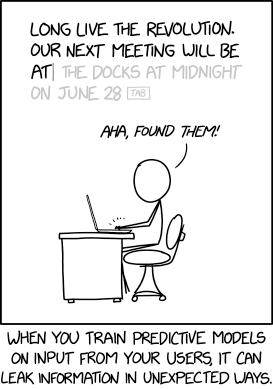
\includegraphics[width=0.20\textwidth, clip]{"./proofs/figures/predictive_models.png"}\\
    \end{center}
  \end{frame}

  \begin{frame}{Anonymiser les données n'est pas suffisant}
    \begin{itemize}
      \item<1->\fullcite{rec26}\\

      \item<2->\fullcite{cell}\\
      
      \item<3->\fullcite{link}
    \end{itemize}

  \end{frame}


  \begin{frame}{\textit{Background} essentiel sur la \textit{differential privacy} (1/4)}
    \begin{itemize}
      \item La \textit{differential privacy} \cite{10.1007/11681878_14} quantifie la perte de confidentialité subit par un individu en participant à une étude. 

      \item<2->\begin{definition}[Jeu de donnés voisins]
          On dit que deux jeux de donnés \(x\) et \(y\) sont voisins et on note \(\dt_{\text{Ham}}(x,y) \leq 1\) s'ils diffèrent sur au plus une entrée \textit{ie} la distance de {\sc Hamming} qui les sépare et majorée par 1.
      \end{definition}
       
      
      \item<3->\begin{definition}[Differential privacy]
          On dit qu'un mécanisme aléatoire\footnote{La notation \(\mathcal X^{(\N)}\) désigne, de manière usuelle, l'ensemble des suites finies de \(\mathcal X\).} \(\mathcal M :\mathcal X^{(\N)} \to \mathcal T\) est \textbf{\((\varepsilon, \delta)\)-\textit{differentially private}} si pour tout \(\mathcal S \subset \mathcal T \) mesurable, 
          \[
              \forall x,y \in \mathcal X^{(\N)} \quad \dt_{\text{Ham}}(x,y) \leq 1 \quad \Rightarrow \quad \mathbb P(\mathcal M(x) \in \mathcal S) \leq \exp(\varepsilon)  \mathbb P(\mathcal M(y) \in \mathcal S) + \delta.
          \] 
          De plus, si \(\delta = 0\), on dit que \(\mathcal M\) est \textbf{\(\varepsilon\)-\textit{differentially private}}. 
      \end{definition}
    \end{itemize}
  \end{frame}

  \begin{frame}{\textit{Background} essentiel sur la \textit{differential privacy} (2/4)}
    \begin{itemize}
      \item<1-> \begin{definition}[Sensibilitée d'une requête]
        Soit \(\mathcal X\) un ensemble, \((\mathcal T, \mathcal N)\) un espace mesuré et \(f : \mathcal X^{(\N)} \to \mathcal T\) une requête. On appel \textbf{sensibilité de \(f\)} la grandeur \(\Delta f\) que l'on définit de la manière suivante:
        \[
            \Delta f = \underset{x, y \in \mathcal X^{(\N)}}{\sup} \left\{ \mathcal N(f(x), f(y)) \ | \ \dt_{\text{Ham}}(x,y) = 1 \right\}. 
        \]
      \end{definition}

      \vspace{-0.5cm}
      \item<2-> \begin{definition}[Mécanisme de {\sc Laplace} \cite{10.1007/11681878_14}]
        Soit \(\mathcal X\) un ensemble de base, \(\varepsilon \in \R_+^\star\), \(n \in \N\) et \(f : \mathcal X^{(\N)} \to \R\) une requête. Notons \(\text{Lap}\) la fonction qui retourne une variable aléatoire suivant la loi de {\sc Laplace}\footnote{Il s'agit de la loi de densité \(x \mapsto 1/(2b) \exp(-|x|/b)\) où \(b\) est le paramètre.} dont la paramètre est l'argument. On appel \textbf{mécanisme de {\sc Laplace}} la fonction 
        \[
            \mathcal M_{f,\varepsilon} : \left\{ 
                \begin{array}{ccc}
                    \mathcal X^{(\N)} & \to & \R\\
                    x & \mapsto & f(x) + \text{Lap}\left( {\Delta f}/{\varepsilon} \right)
                \end{array}
            \right.    
        \]
      \end{definition}
    \end{itemize}
  \end{frame}

  \begin{frame}{\textit{Background} essentiel sur la \textit{differential privacy} (3/4)}
    \begin{definition}[Mécanisme de {\sc Laplace} \cite{10.1007/11681878_14}]
      Soit \(\mathcal X\) un ensemble de base, \(\varepsilon \in \R_+^\star\), \(n \in \N\) et \(f : \mathcal X^{(\N)} \to \R\) une requête. Notons \(\text{Lap}\) la fonction qui retourne une variable aléatoire suivant la loi de {\sc Laplace} dont la paramètre est l'argument. On appel \textbf{mécanisme de {\sc Laplace}} la fonction 
      \[
          \mathcal M_{f,\varepsilon} : \left\{ 
              \begin{array}{ccc}
                  \mathcal X^{(\N)} & \to & \R\\
                  x & \mapsto & f(x) + \text{Lap}\left( {\Delta f}/{\varepsilon} \right)
              \end{array}
          \right.    
      \]
    \end{definition}

    \begin{theorem}
      Le mécanisme de {\sc Laplace} est \textit{differentially private}.
  \end{theorem}
  \end{frame}

  \begin{frame}{\textit{Background} essentiel sur la \textit{differential privacy} (4/4)}
    \begin{itemize}
      \item<1-> \begin{theorem}[Théorème de composition (simple) \cite{10.1007/11681878_14}]
          \label{compo}
          Soit \(\mathcal X\) un ensemble de base, \(n \in \N\) un nombre de mécanismes, \((\mathcal T_i)_{i \leq n}\) des ensembles d'arrivé et \((\mathcal M_i : \mathcal X^{(\N)} \to \mathcal T_i)_{i \leq n}\) des mécanismes mutuellement indépendants respectivement \(\varepsilon_i\)-\textit{differentially private}. L’exécution des \(n\) mécanismes est \(\left(\sum\limits_{i = 1}^n \varepsilon_i\right)\)-\textit{differentially private}.
        \end{theorem} 
        \vspace{-0.3cm}
      \item<2> \begin{proof}
          Considérons \((\mathcal S_i)_{i \leq n} \subset \prod_{i = 1}^n \mathcal T_i\) et \(x, x' \in \mathcal X^{(\N)}\) tel que \(\dt_{\text{Ham}(x,x') \leq 1}\).
          \[
              \begin{array}[]{rcl}
                  \mathbb P\left(\mathcal M_1(x) \in \mathcal S_1 \ \wedge \ \mathcal M_2(x) \in \mathcal S_2 \ \wedge \dots \right) & \overset{\text{indé.}}{=} & \prod_{i = 1}^n \mathbb P\left(\mathcal M_i(x) \in \mathcal S_i \right)\\
                  & \overset{\text{DP}}{\leq} & \prod_{i = 1}^n e^{\varepsilon_i}\mathbb P\left(\mathcal M_i(x') \in \mathcal S_i \right)\\
                  & \overset{\text{indé.}}{=} & e^{\sum_{i = 1}^n \varepsilon_i}\mathbb P\left(\mathcal M_1(x') \in \mathcal S_1 \ \wedge \dots \right)
              \end{array}
          \]
        \end{proof}
    \end{itemize}
  \end{frame}

  \begin{frame}{L'échec de la méthode naïve}
    \begin{itemize}
      \item<1-> Soit \(x \in [0,1]^n\). On a \(\Delta\text{méd} = 1\).\\
      \only<1>{\begin{center}
        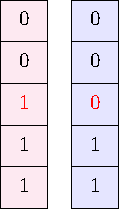
\includegraphics[width=0.30\textwidth, clip]{"./proofs/figures/6HBRJaKv0r342kYs.pdf"}
      \end{center}
      }
      \item<2->  Or,   \[
        |\text{méd}(x) - \mathcal M_{\text{méd}, \varepsilon}| = |\text{Lap}(1/\varepsilon)|.    
      \] 

      \item<3->  D'où,  \begin{align*}
          \mathbb E\left( |\text{méd}(x) - \mathcal M_{f, \varepsilon}| \right) & = \int_{\R} \mathbb P \left( |\text{Lap}(1/\varepsilon)| > t \right) \dt t = \int_{\R_+} e^{-\varepsilon t}  \dt t = \dfrac{1}{\varepsilon}.
        \end{align*} 

      \item<4-> Néanmoins nous avons forcement \(\text{méd}(x) \in [0,1]\). \textbf{Cette méthode ne peut donc pas convenir}.
    \end{itemize}
  \end{frame}




\section{Méthode des histogrammes}
  \begin{frame}[containsverbatim]{AboveThreshold \cite{10.1007/11681878_14}}
    \begin{code}
  AboveThreshold(database, queries, threshold, epsilon){
    Assert("les requêtes sont toutes de sensibilité 1");
    result = 0;
    noisyThreshold = threshold + Lap(2/epsilon);
    for(querie in queries){
        nu = Lap(4/epsilon);
        if(querie(D) + nu > noisyThreshold)
            return result;
        else
            ++result; 
    }
    return -1; /* Aucune requête n'a dépassé le seuil */
  }
    \end{code}
    \begin{theorem}
      \mintinline{cpp}{AboveThreshold} est \(\varepsilon\)-\textit{differentially private}.
    \end{theorem}
  \end{frame} 

  \begin{frame}[containsverbatim]{Présentation de la méthode des histogrammes}
    \begin{code}
  HistogramMethod(database, epsilon, a, b){
    steps = 1.5*n/log(n);
    epsilon /= 9; /* composition theorem */
    result = {};
    for(d in {1 ... 9}){ /* which decile */
        T = d*card(database)/10;
        for(i in {1 ... steps}){
            fi = x -> card({element in x | element < i*(b-a)
                                                      /steps});
            queries.push_back(fi);
        }
        T = d*card(database)/10;
        result.push_back(AboveThreshold(database, queries, T, 
                                    epsilon)*(b-a)/steps});
    }
    return result;
  }
    \end{code}

    % \begin{theorem}
    %   \mintinline{cpp}{HistogramMethod} est \(\varepsilon\)-\textit{differentially private}.
    % \end{theorem}
  \end{frame}

  \begin{frame}{Analyse de précision - le cas de la loi uniforme standard (1/5)}
    \only<1>{\begin{definition}[Fonction Beta incomplète (régularisée)]
      On appel respectivement fonction beta incomplète et fonction beta incomplète régularisée les fonctions 
      \begin{align*}
        \Beta : & \left\{ 
          \begin{array}[]{ccc}
              [0,1] \times (\R_+^\star)^2 & \to & \R_+\\
              (x, \alpha, \beta) & \mapsto & \displaystyle\int_0^x t^{\alpha - 1} (1 - t)^{\beta -1} \dt t
          \end{array}
      \right.\\ 
      I_\bullet : & \left\{ 
          \begin{array}[]{ccc}
              (\R_+^\star)^2 & \to & \R_+\\
              (\alpha, \beta) & \mapsto & \dfrac{B(\bullet, \alpha, \beta)}{B(1, \alpha, \beta)}
          \end{array}
      \right.  .
      \end{align*}
    \end{definition}}

    \only<2>{\begin{definition}[Fonction Beta incomplète (régularisée)]
      On appel respectivement fonction beta incomplète et fonction beta incomplète régularisée les fonctions 
      \[
          \Beta : (x, \alpha, \beta) \mapsto \displaystyle\int_0^x t^{\alpha - 1} (1 - t)^{\beta -1} \dt t
           \quad \text{et} \quad  I_\bullet : (\alpha, \beta) \mapsto  \dfrac{B(\bullet, \alpha, \beta)}{B(1, \alpha, \beta)}.
      \]
    \end{definition}}
    
    \only<2>{\begin{definition}[Loi beta]
        On appel loi beta de paramètre \((\alpha, \beta) \in \R_+^\star\) la loi de densité
        \[
                f_{\alpha,\beta} : [0,1] \ni x \mapsto \dfrac{x^{\alpha - 1} (1-x)^{\beta} - 1}{B(1, \alpha, \beta)}
        \]
    \end{definition}}
  \end{frame}

  \begin{frame}{Analyse de précision - le cas de la loi uniforme standard (2/5)}
    \begin{definition}[Statistique d'ordre]
      Soit \(X\) un échantillon statistique de cardinal \(n \in \N\). Pour tout \(k \in \inte 1 n \) on note \(X_{(i)}\) et on appel \textbf{statistique d'ordre} de rang \(k\) la \(k\)-ème plus petite valeur de l'échantillon.
    \end{definition}

    \begin{theorem}[Loi des statistiques d'ordre d'un échantillon issue de \(\mathcal U(0,1)\)]
        \label{staorduni}
        Soit \(X\) un ensemble de \(n\) variables aléatoires \((X_i)_i\) indépendantes et suivant toutes la loi uniforme sur [0,1] et \(k \in \inte 1 n \). La \(k\)-ème statistique d'ordre de \(X\), \(X_{(k)}\), est distribuée suivant la loi beta de paramètre \((k, n-k+1)\).
    \end{theorem}
  \end{frame}

  \begin{frame}{Analyse de précision - le cas de la loi uniforme standard (3/5)}
    \begin{theorem}[Précision moyenne de \mintinline{cpp}{HistogramMethod}]\label{pmhm}
      Soit \(X\) un ensemble de \(n\) (tel que \(8\log(3n/(\beta\log n))/\varepsilon) \leq n/10\)) variables aléatoires \((X_i)_i\) indépendantes et suivant toutes la loi uniforme standard. Soit \(i \in \inte 1 9 \). Notons \((d_i^l)_i\) les déciles de la loi. Posons \(A\) la variable aléatoire \mintinline{cpp}{HistogramMethod(X, epsilon, 0, 1)} et \(\alpha = 8\log(3n\sqrt n)/\varepsilon)\). On a 
      \vspace{-0.3cm}
      \begin{align*}
          \mathbb E\left( |A_i - d_i^l| \right) & \leq \int_{0}^{d_i^l}\left( 1 - I_{d_i^l + t}(\lceil in/10 + \alpha\rceil, n - \lceil in/10 + \alpha \rceil + 1) \right) \dt t\\
          &\quad + \int_{0}^{d_i^l}I_{d_i^l - t}(\lfloor in/10 - \alpha \rfloor , n - \lfloor in/10 - \alpha \rfloor + 1) \dt t + \beta \\
          &\quad + I_{d_i^l - 0.1}(\lfloor in/10 - \alpha \rfloor , n - \lfloor in/10 - \alpha \rfloor + 1)\\
          &\quad + I_{1 - d_i^l - 0.1}(n - \lceil in/10 + \alpha \rceil + 1, \lceil in/10 + \alpha\rceil)\\
          &\quad + \dfrac{2\log n}{3n} + d_i^l\beta.
      \end{align*}
    \end{theorem}
  \end{frame}

  \begin{frame}{Analyse de précision - le cas de la loi uniforme standard (4/5)}
    \begin{corollary}[(im)Précision moyenne de \mintinline{cpp}{HistogramMethod}]
      \label{coro_err_quadra}
      Soit \(X\) un ensemble de \(n\) (tel que \(8\log(3n\sqrt n))/\varepsilon) \leq n/10\)) variables aléatoires \((X_i)_i\) indépendantes et suivant toutes la loi uniforme standard. Soit \(i \in \inte 1 9 \). Notons \((d_i^l)_i\) les déciles de la loi. Posons \(A\) la variable aléatoire \mintinline{cpp}{HistogramMethod(X, epsilon, 0, 1)}, \(\alpha = 8\log(3n\sqrt n)/\varepsilon)\). On a 
      \vspace{-0.3cm}
      \begin{align*}
          \mathbb E\left( |A_i - d_i^l| \right) & \leq \int_{0}^{d_i^l}\left( 1 - I_{d_i^l + t}(\lceil in/10 + \alpha\rceil, n - \lceil in/10 + \alpha \rceil + 1) \right) \dt t\\
          &\quad + \int_{0}^{d_i^l}I_{d_i^l - t}(\lfloor in/10 - \alpha \rfloor , n - \lfloor in/10 - \alpha \rfloor + 1) \dt t + \dfrac{1}{\sqrt n \log n}\\
          &\quad  + I_{d_i^l - 0.1}(\lfloor in/10 - \alpha \rfloor , n - \lfloor in/10 - \alpha \rfloor + 1)\\
          &\quad + I_{1 - d_i^l - 0.1}(n - \lceil in/10 + \alpha \rceil + 1, \lceil in/10 + \alpha\rceil)\\
          &\quad  + \dfrac{2\log n}{3n} + \dfrac{d_i^l}{\sqrt n \log n}.
      \end{align*}
    \end{corollary}
  \end{frame}

  \begin{frame}{Analyse de précision - le cas de la loi uniforme standard (5/5)}
    \begin{theorem}[(im)Précision moyenne de \mintinline{cpp}{HistogramMethod}]
      Soit \(X\) un ensemble de \(n\) (tel que \(0\leq 8\log(3n\sqrt n)/\varepsilon) \leq n/10\)) variables aléatoires \((X_i)_i\) indépendantes et suivant toutes la loi uniforme sur [0,1]. Soit \(i \in \inte 1 9 \) et \(k \in \N\). Notons \((d_i)_i\) les décile de la loi. Posons \(A\) la variable aléatoire  \mintinline{cpp}{HistogramMethod(X, epsilon, 0, 1)} et \(\alpha = 8\log(3n\sqrt n)/\varepsilon)\). On a,
      \begin{align*}
          \mathbb E\left( |A_i - d_i^l| \right) & \leq 2\sqrt{\dfrac{\pi}{2n}} + \dfrac{d_i^l + 1}{\sqrt n \log n} + \dfrac{\log n}{n}\left( \dfrac{2}{3} + \dfrac{16}{\varepsilon}\log(3) \right)\\
          & \quad + 2\exp\left( -2n\left(0.1 - \dfrac{\alpha}{n}\right)^2 \right).
      \end{align*}
    \end{theorem}
  \end{frame}

\section{Le mécanisme de sensibilité inverse}
  \begin{frame}{Présentation du mécanisme (1/2)}
    \begin{definition}[Longueur]
      Soit \(x \in \mathcal X^{(\N)}\), \(f : \mathcal X^{(\N)} \to \mathcal T\) et \(t \in \mathcal T\). La longueur est le nombre minimum de valeurs à modifier dans \(x\) pour obtenir \(x'\) tel que \(f(x') = t\). On a 
      \[
          \len_f(x,t) := \inf_{x' \in \mathcal X^{(\N)}}\left\{|| x - x'||_1 \ |\ f(x') = t \right\}.
      \]
    \end{definition}
    
    \begin{definition}[Mécanisme de sensibilité inverse \cite{Asi2020NearII}]
        Soit \(f : \mathcal X^{(\N)} \to \mathcal T\) et \(\varepsilon \in \R_+\). Pour une mesure \(\mu\) sur \(\mathcal T\), on définit le mécanisme aléatoire \(\mathcal M(x)\) par sa fonction de densité 
        \[
            t \mapsto \dfrac{\exp(-\len_f(x, t)\varepsilon/2)}{\int_\mathcal T \exp(-\len_f(x, s)\varepsilon/2)\dt \mu(s)}.
        \] 
    \end{definition}
  \end{frame}

  \begin{frame}{Présentation du mécanisme (2/2)}
    \begin{definition}[Longueur lisse]
      Soit \(x \in \mathcal X^{(\N)}\), \(f : \mathcal X^{(\N)} \to \mathcal T\) et \(\rho \in \R_+\). Si \(\mathcal N\) est une norme sur \(\mathcal T\),
      \[
          \len_f^{\rho} : 
          \left\{
              \begin{array}[]{rcl}
                  \mathcal T & \to & \N\\
                  t & \mapsto & \inf_{s \in \mathcal T, \mathcal N(s,t) \leq \rho}\left\{\len_f(x,s) \right\}  
              \end{array}
          \right. .   
      \]
    \end{definition}
    
    \begin{definition}[Mécanisme de sensibilité inverse \(\rho\)-lisse \cite{Asi2020NearII}]
        Soit \(f : \mathcal X^{(\N)} \to \mathcal T\) et \(\rho, \varepsilon \in \R_+\). Pour une mesure \(\mu\) sur \(\mathcal T\), on définit le mécanisme aléatoire \(\mathcal M_{\text{cont}}(x)\) par sa fonction de densité 
        \[
            t \mapsto \dfrac{\exp(-\len_f^\rho(x, t)\varepsilon/2)}{\int_\mathcal T \exp(-\len_f^\rho(x, s)\varepsilon/2)\dt \mu(s)}.   
        \] 
    \end{definition}
  \end{frame}

  \begin{frame}{Analyse de complexité}
    \begin{center}
      \begin{itemize}
        \item<1->{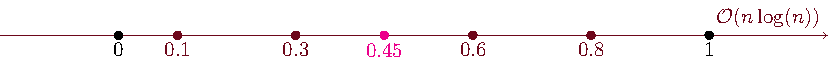
\includegraphics[width=0.90\textwidth, clip]{"./presentation/figures/step1.pdf"}}\vspace{0.8cm}
        \item<2->{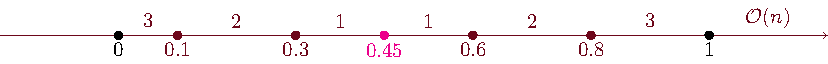
\includegraphics[width=0.90\textwidth, clip]{"./presentation/figures/step2.pdf"}}\vspace{0.8cm}
        \item<3->{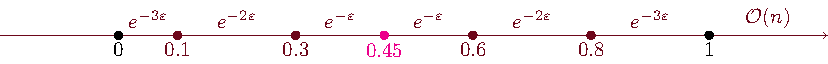
\includegraphics[width=0.90\textwidth, clip]{"./presentation/figures/step3.pdf"}}\vspace{0.8cm}
        \item<4->{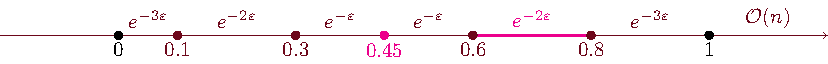
\includegraphics[width=0.90\textwidth, clip]{"./presentation/figures/step4.pdf"}}\vspace{0.8cm}
      \end{itemize}
    \end{center}

    La complexité de l'algorithme est donc au pire en \(\mathcal O(n\log(n))\).
  \end{frame}

  \begin{frame}{Précision pour l'estimation de déciles}

  \end{frame}

\section{Comparaison entre le mécanisme de sensibilité inverse et la méthode des histogrammes}
  \begin{frame}{Comparaison des bornes obtenues}

  \end{frame}

  \begin{frame}{Résultats expérimentaux}

  \end{frame}

\section{Conclusion}
  \begin{frame}{Conclusion}

  \end{frame}

\section{Références}

  \begin{frame}{Référence}
    \printbibliography
  \end{frame}


\end{document}
